\documentclass[crop,tikz]{standalone}
\usepackage{mathrsfs} % for mathscr to work
\usetikzlibrary{shapes,arrows}
\usetikzlibrary{calc}
\usepackage{amsmath}
\newcommand{\fb}{\bar{f}}
\newcommand{\gb}{\bar{g}}
\newcommand{\ds}{\displaystyle}
\newcommand{\Hs}{\mathscr{H}} % Hscore
\newcommand{\Hnest}{\Hs^{\perp}}
\newcommand{\pplus}{\mathbin{+\mkern-10mu+}} % concatenate
\newcommand{\con}{\Large $\pplus$}

\tikzset{%
  bullet/.style={scale = .8}, % yshift = -.7mm, 1.5
  extfill/.style={fill = red!30, fill opacity = .2}, % color
  frozenfill/.style={fill = gray, fill opacity = .2}, % gray
  ext/.style={trapezium, trapezium angle=67.5, draw, % extractor
  inner ysep=5pt, outer sep=0pt, extfill,
  minimum height=1.2cm, minimum width=0pt},
  extl/.style={isosceles triangle,
    isosceles triangle apex angle=60, minimum height=1.2cm,
    draw, extfill, minimum height=1.2cm, minimum width=0pt}, % linear ext
  block/.style    = {draw, thick, rectangle, minimum height = 3em, minimum width = 5em},
  sum/.style      = {draw, circle, node distance = 2cm}, % Adder
  con/.style      = {draw, circle, node distance = 2cm}, % concatenate
  input/.style    = {coordinate}, % Input
  int/.style    = {coordinate}, % intersection
  missing/.style={
    draw=none,
    fill=none,
    yshift = 0.1cm,
    scale = 1.5,
%    scale=1,
%    text height=0.333cm,
    execute at begin node={\color{black}{$\vdots$}}
  },
  output/.style   = {coordinate}, % Output
  exts/.style={ext, 
  minimum height=1cm},
}

\begin{document}%Modified from: %https://texample.net/tikz/examples/noise-shaper/
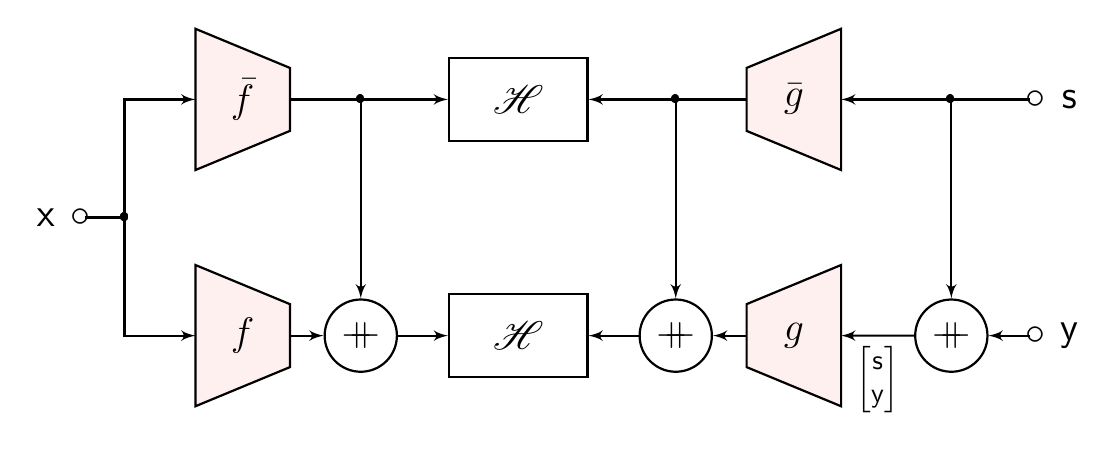
\begin{tikzpicture}[auto, thick, node distance=2cm, >=latex'%stealth% >=triangle 45
  ]
  % draw H-score's
  \foreach \i [count = \y] in {1, 2}
  \draw node [block] (H-\i) at (6.5, -3 * \y cm) {\Large $\Hs$};

  \foreach \i in {1, 2}
  {
  \draw node [ext, left of = H-\i, node distance=3.5cm, rotate = -90] (f-\i)  {};
  \draw node [ext, right of = H-\i, node distance=3.5cm, rotate = 90] (g-\i)  {};
}


    \draw node at (f-1)  {\Large $\fb$}
    node at (g-1)  {\Large $\gb$};

    \draw node at (f-2)  {\Large $f$}
        node at (g-2)  {\Large $g$};

        \draw
        node [con, left of = H-2, node distance = 2cm] (conl) {\con}
        node [con, right of = H-2, node distance = 2cm] (conr) {\con};

% \draw node [extl, left of = H-2, node distance=4.72cm] {};
\draw [->] (f-1) -- (H-1);
\draw [->] (g-1) -- (H-1);

\draw [->] (f-2) -- (conl);
\draw [->] (g-2) -- (conr);
\draw [->] (conl) -- node[below] {% $\ds 
%           \begin{bmatrix}
%             \fb\\
%             f
%           \end{bmatrix}
% $
}(H-2);
\draw [->] (conr) -- node[below] {% $\ds 
%           \begin{bmatrix}
%             \gb\\
%             g
%           \end{bmatrix}
% $
}(H-2);


\draw [->] (f-1) -| (conl);
\draw [->] (g-1) -| (conr);
\draw node at (conl |- f-1) [bullet] {\textbullet} ;
\draw node at (conr |- g-1) [bullet] {\textbullet} ;


\draw node [input] (x) at (1,-4.5) {}
     node [xshift = -0.5cm] at (x) {\Large $\mathsf x$}
     node [xshift = -0.6mm] at (x) {\Large $\circ$};

     \draw node [input] (s) at (13,-3) {}
     node [xshift = 0.5cm] at (s){\Large $\mathsf s$} 
     node [xshift = 0.7mm] at (s) {\Large $\circ$} ;
         \draw node [input] (y) at (13,-6) {} %.3
         node [xshift = 0.5cm] at (y){\Large $\mathsf y$} 
         node [xshift = 0.7mm] at (y) {\Large $\circ$} ;

         \draw node [con, left of = y, node distance=1cm, xshift = -0 cm] (con-ys)  {\con};

  \foreach \i [count = \y] in {1, 2}  
\draw [->] (x) -- + (.5, 0) node [bullet] {\textbullet} |- (f-\i);
  
\draw [->] (s) |- (g-1);

  \draw [->] (s) -| (con-ys);
  \draw [->] (y) -- (con-ys);
  \draw [->] (con-ys) -- node[below] {
    $\ds 
          \begin{bmatrix}
            \mathsf s\\
            \mathsf y
          \end{bmatrix}
          $} (g-2);

    \draw node at (con-ys |- s) [bullet] {\textbullet} ;
  % \draw [->] (y) -- + (-.5, 0) node [bullet] {\textbullet} |- (g-\i);

\end{tikzpicture}

\end{document}

%%% Local Variables:
%%% mode: latex
%%% TeX-master: t
%%% End:
